\chapter*{Problema A - ¡Arriba, Papalotes, Arriba!}

Queremos hacer papalotes triangulares y tú nos
ayudarás. Para eso tenemos 5 varas de madera que nos
servirán a darle forma al papalote como nosotros 
lo deseamos. 

La siguiente figura nos ayudará a ilustrarte el tipo
de papalotes que pretendemos hacer.

\begin{center}
    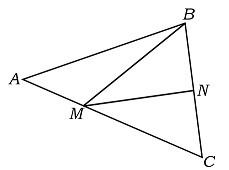
\includegraphics{images/Triangulo.jpg}
\end{center}

Tres de las varas con las que contamos ($AB$, $BC$ y 
$CA$) las usaremos para delimitar la figura del 
triángulo; una más se colocará a partir del vértice 
$B$ hacia algún punto $M$ del lado opuesto; la 
última irá del punto $M$ hacia algún punto $N$ sobre
el segmento $BC$.

Necesitamos cortar el material que va en los 
triángulos ABM, BMN y CMN,
y debemos ser muy cuidadosos para crear bellos 
papalotes. Obtener el área de los mencionados 
triángulos será tu trabajo.

¡Ah! Una cosa más. Te daré un dato que tal vez pueda
serte útil. El área de un triángulo se puede obtener
con la siguiente fórmula:
$$A = \sqrt{S \cdot (S-a) \cdot (S-b) \cdot (S-c)}$$
donde $a, b$ y $c$ son los lados del triángulo y $S$ es
su semiperímetro.




\subsection*{Entrada}
La primera línea de la entrada contendrá un número $T$, 
el número de casos. Luego vendrán $T$ líneas -una para
cada caso; cada una estará compuesta por 5 números 
reales positivos separados por un espacio, que 
representarán la longitud de los segmentos $AB$, $BC$,
$CA$, $MC$ y $NC$, en ese orden.




\subsection*{Salida}
Imprime las áreas de los tres triángulos en orden 
ascendente, cada área en una línea distinta. Repite
el proceso para cada caso.

Tendrás un margen de error $10^{-5}$.



\subsection*{Límites de los conjuntos de datos}

\begin{itemize}
    \item Grande: $ \;\, 1 \leq T \leq 10^{3}$, 
    $0 < AB, BC, CA, MC, NC \leq 100$ $\quad \;\,$ $100$ puntos.
\end{itemize}



\begin{multicols}{2}

\subsection*{Entrada Ejemplo}

\begin{verbatim}
1
13 4 15 6 1
\end{verbatim}

\columnbreak

\subsection*{Salida Ejemplo}

\begin{verbatim}
2.4
7.2
14.4
\end{verbatim}

\end{multicols}